\subsection{Webanalysetools und das Kantonale Datenschutzgesetz}
Da sich Webanalysetools 
\subsection{}

\subsection{Marktangebot - Webanalysetools}

Webanalysetools lassen sich aufgrund von verschiedenen Charakteristiken Gruppieren.
Eine übliche Gruppierung basiert auf der Methode der Datensammlung. Diese lässt sich im wesentlichen auf vier verschiedene Arten durchführen \parencite{nakatani2011toolselectionmethod}:

\begin{enumerate}
    \item Web Beacon - Bei Web Beacons handelt es sich um kleine Bilddateien, welche sich auf einer Webseite eingefügt werden können und per Request angefordert werden. Sie ermöglichen es, durch das zählen der Downloads dieses Beacons, die Anzahl Hits von Seiten oder sogar Unterseiten aufzuzeichnen. Web Beacons werden in der Praxis oft als Teil von Page Tagging eingesetzt. \parencite[S. 173]{nakatani2011toolselectionmethod}.
    \item Packet Sniffing - Durch das Abfangen und analysieren der Webpakete auf dem Webserver, können mit Packet Sniffing Daten gesammelt werden. Packet Sniffing findet in der Praxis hauptsächlich Anwendung bei multivariatem Testen \parencite[S. 4]{waisberg2009webShort}.
    \item Transaktionsloganalyse - Bei dieser Methode werden die Log Dateien auf dem Webserver analysiert. Transaktionsloganalyse ist eine in der Praxis nach wie vor viel verwendete Methode, um Daten über Seitenaufrufe zu sammeln.\parencite[S. 173]{nakatani2011toolselectionmethod}. Die Tiefe der Daten die jedoch gesammelt werden kann hält sich jedoch in Grenzen. 
    \item Page Tagging - \parencite[S. 173]{nakatani2011toolselectionmethod}
  \end{enumerate}

\subsection{}
\subsection{}
\subsection{}
\subsection{}


Results - \ref{fig: a black image}

\begin{figure}[h]
    \centering
    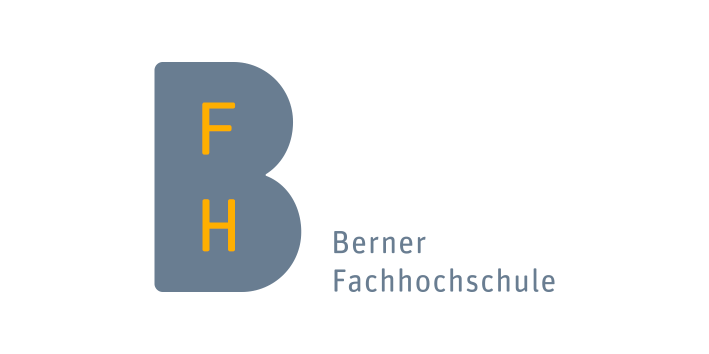
\includegraphics{BFH.png}
    \caption{Example image}
    \label{fig: a black image}
\end{figure}
